
% Chapter 3

\chapter{État de l'art} % 3rd chapter title

\label{Chapter3} % For referencing the chapter elsewhere, use \ref{Chapter3} 


%----------------------------------------------------------------------------------------

\section{Position du problème}

Nous commensons par présenter une modélisation mathématique d'une plaque de glace (appelé floe) sur la mer. Six variables sont nécésaires pour décrire un floe sur la mer (voir figure 1): 
\begin{itemize}
    \item Un ouvert connexe $\omega \in \Rdeux$ décrivant la section longitidunale du floe;
    \item Deux fonction $\hplus, \hmoins \in \mathcal{F}(\omega, \Run)$ décrivant l'épasseur du floe, telle que $\forall x \in \omega, \hmoins(x) \leq \hplus(x)$;
    \item Le centre de gravité du floe $G(w)$;
    \item Deux vecteurs $e_1(\omega)$ et $e_2(\omega)$ formant une base sur $\omega$.
\end{itemize}

\begin{figure}[H]
    \centering
    \begin{subfigure}[b]{0.45\textwidth}
        \centering
        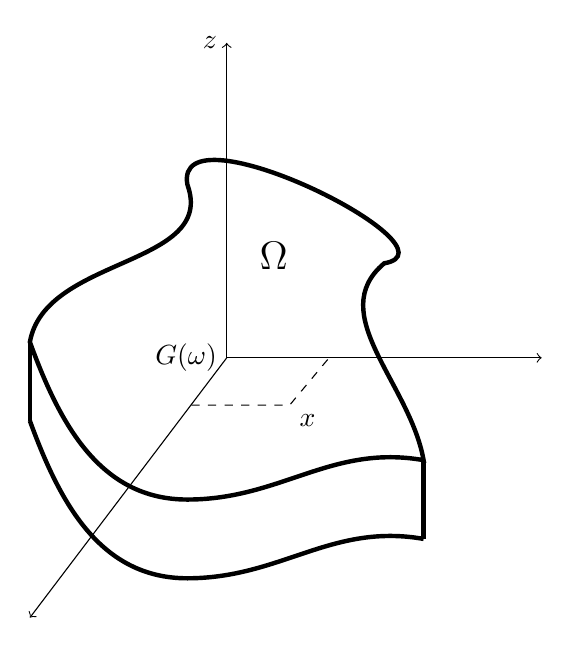
\begin{tikzpicture}
\node[coordinate] (v1) at (-3,3) {};
\node[coordinate] (v2) at (-5,1) {};
\node[coordinate] (v3) at (-3,-1) {};
\node[coordinate] (v4) at (0,-0.5) {};
\node[coordinate] (v5) at (-0.5,2) {};
%\draw  plot[smooth cycle, tension=.7] coordinates {(v5) (v1) (v2) (v3) (v4) (v5)};

\draw [ultra thick] (v1) to [out=290, in=80] (v2) to[out=290, in=180] (v3) to[out=0,in=170] (v4) to[out=100,in=220] (v5) to[out=10,in=100] (v1);

\node[coordinate] (v6) at (-5,0) {};
\node[coordinate] (v7) at (-3,-2) {};
\node[coordinate] (v8) at (0,-1.5) {};

\draw [ultra thick] (v2)--(v6); \draw [ultra thick] (v4)--(v8);
\draw [ultra thick]  (v6) to[out=290, in=180] (v7) to[out=0,in=170] (v8);

\node[coordinate] (v9) at (-2.5,0.8) {};
\node[coordinate] (v10) at (-5.0,-2.5) {};
\node[coordinate] (v11) at (1.5,0.8) {};
\node[coordinate] (v12) at (-2.5,4.8) {};

\draw [->] (v9)--(v10);
\draw [->] (v9)--(v11);
\draw [->] (v9)--(v12);


\node[left] (v9) at (-2.5,0.8) {$G(\omega)$};
\node[left] (v12) at (-2.5,4.8) {$z$};
\node[above left] (v13) at (-1.6,1.8) {\Large $\Omega$};

\node[coordinate] (v14) at (-1.2,0.8) {};
\node[coordinate] (v15) at (-1.7,0.2) {};
\node[coordinate] (v16) at (-2.95,0.2) {};
\draw[dashed] (v16)--(v15)--(v14);

\node[below right] (v15) at (-1.7,0.2) {$x$};

\end{tikzpicture} 
        \caption{Vue d' un floe}
        % \label{fig:floe1}
    \end{subfigure}
    \hfill
    \begin{subfigure}[b]{0.45\textwidth}
        \centering
        \usetikzlibrary{patterns}

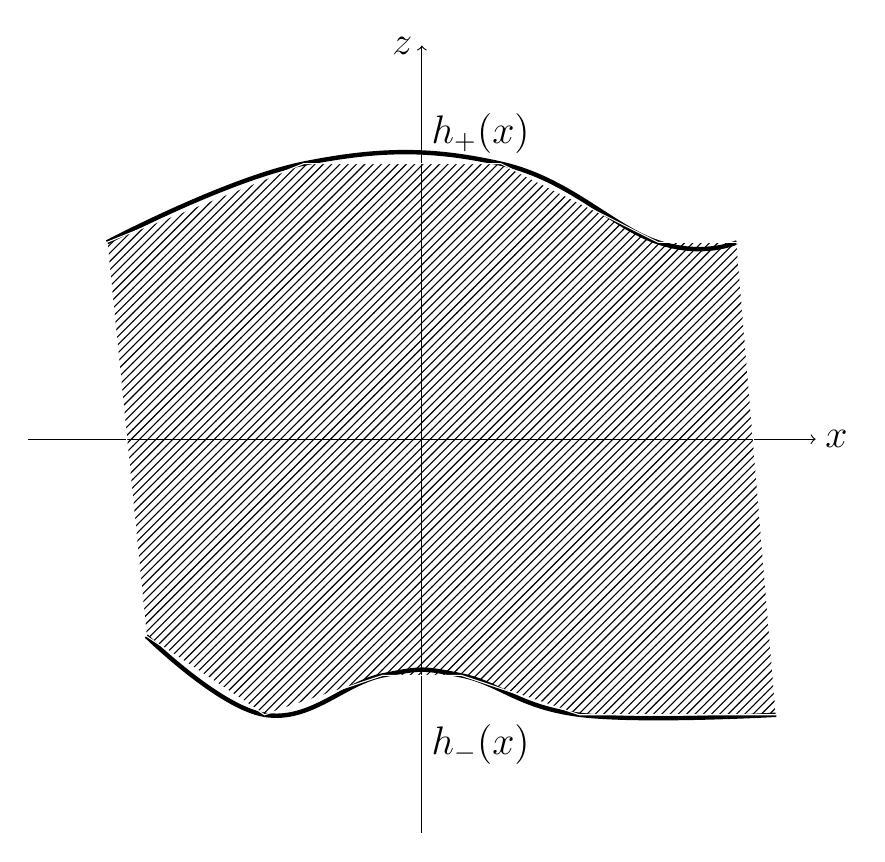
\begin{tikzpicture}

\node[coordinate] (v0) at (0,0) {};
\node[coordinate] (v1) at (-5,0) {};
\node[coordinate] (v2) at (5,0) {};
\node[coordinate] (v3) at (0,-5) {};
\node[coordinate] (v4) at (0,5) {};

\draw [->] (v1)--(v2);
\draw [->] (v3)--(v4);

\node (v5) at (-4,2.5) {};
\node (v6) at (-1.5,3.5) {};
\node (v7) at (1,3.5) {};
\node (v8) at (3,2.5) {};
\node (v9) at (4,2.5) {};
\node (v10) at (-3.5,-2.5) {};
\node (v11) at (-2,-3.5) {};
\node (v12) at (-0.5,-3) {};
\node (v13) at (0.5,-3) {};
\node (v14) at (2,-3.5) {};
\node (v15) at (4.5,-3.5) {};

\draw[ultra thick]  plot[smooth, tension=.7] coordinates {(v5) (v6) (v7) (v8) (v9)};
\draw[ultra thick]  plot[smooth, tension=.7] coordinates {(v10) (v11) (v12) (v13) (v14) (v15)};

\draw [white, pattern=north east lines, xshift=0.5cm,yshift=4.5cm] plot coordinates {(v5) (v6) (v7) (v8) (v9) (v15) (v14) (v13) (v12) (v11) (v10) (v5)};

\node [above right] at (0,3.5) {\Large \bfseries $h_{+}(x)$};
\node [below right] at (0,-3.5) {\Large \bfseries $h_{-}(x)$};
\node [right] at (5,0) {\Large \bfseries $x$};
\node [left] at (0,5) {\Large \bfseries $z$};

\end{tikzpicture} 
        % \includegraphics[width=2cm]{Figures/FloeVue2.tex}
        \caption{Coupe transversale}
        \label{fig:flo2}
    \end{subfigure}
       \caption{Illustration de la géométrie d'un floe de glace $\Omega$.}
       \label{fig:floe}
\end{figure}

Le volume $\Omega$ du floe est donné par:
\[
    \Omega = \{(x,z) | x \in \omega \in \Rdeux, z \in ]\hmoins(x), \hplus(x)[ \} \,.
\] 
Les fonctions $\hmoins$ et $\hplus$ permettent de définir trois quantités (voir figure 2):
\begin{itemize}
    \item L'épaisseur moyenne du floe : $\bar{h} =  \sup_{x\in\omega}{\hplus(x)} - \inf_{x\in\omega}{\hmoins(x)}$;
    \item La plus forte epaisseur : $\bar{h}^* = \sup_{x\in\omega}{ \vert \hplus(x) - \hmoins(x) \vert}$. 
    \item La plus faible epaisseur : $\underline{h}^* = \inf_{x\in\omega}{ \vert \hplus(x) - \hmoins(x) \vert} $. 
\end{itemize}

\begin{figure}
    \centering
    % \begin{tikzpicture}
	\begin{pgfonlayer}{nodelayer}
		\node [style=none] (0) at (0, 0) {};
		\node [style=none] (1) at (0, 5) {};
		\node [style=none] (2) at (0, -5) {};
		\node [style=none] (3) at (10, 0) {};
		\node [style=none] (4) at (-10, 0) {};
		\node [style=none] (5) at (-9.25, 2.5) {};
		\node [style=none] (6) at (-3.5, 1.5) {};
		\node [style=none] (7) at (3.25, 1.25) {};
		\node [style=none] (8) at (8.75, 4.75) {};
		\node [style=none] (9) at (-9, -6.75) {};
		\node [style=none] (10) at (-5, -4) {};
		\node [style=none] (11) at (2.5, -1.75) {};
		\node [style=none] (12) at (8.75, -1.25) {};
	\end{pgfonlayer}
	\begin{pgfonlayer}{edgelayer}
		\draw [->] (1.center) to (2.center);
		\draw [->] (4.center) to (3.center);
		\draw [bend right=15, looseness=0.75] (5.center) to (6.center);
		\draw [in=-165, out=0, looseness=1.25] (6.center) to (7.center);
		\draw [in=-135, out=15, looseness=1.25] (7.center) to (8.center);
		\draw [in=-165, out=45] (9.center) to (10.center);
		\draw [in=195, out=0, looseness=0.50] (10.center) to (11.center);
		\draw [in=180, out=15, looseness=0.75] (11.center) to (12.center);
	\end{pgfonlayer}
\end{tikzpicture}

    \includegraphics[width=.4\textwidth]{h.tikz}
\end{figure}

\textit{FIGURE 2 ICI. Afin d'obtenir un floe floes relativement plats; Aussi, $\hmoins$ sera pris identiquement nul, et $\hplus$ constant. }

Les vecteur $e_1(\omega)$ et $e_2(\omega)$ sont liés à $\omega$, et pointent vers un point fixe du bord $\partial \omega$ du floe i.e:
\[
    \exists \sigma_i \in \partial \omega | e_i(\omega) = \frac{\sigma_i - G(\omega)}{\Vert \sigma_i - G(\omega) \Vert}, \text{ pour } i \in \{1,2\} \,,
\]
où $\Vert \cdot \Vert$ désigne la norme euclidienne de $\Rdeux$. Notons que $\sigma_1 \neq \sigma_2$, et $\eun \cdot \edeux = 0$ de facon à ce que la base $(\eun, \edeux)$ soit directe.

Un floe $F = (\omega, \eun, \edeux, G(\omega), \hmoins, \hplus)$ se déplace sur la mer\footnote{Pour l'instant, la mer est considérée comme un ouvert dans $\Rdeux$. Plus tard, nous prendrons en compte sont épaisseur lorsque nous modelserons la mer par une sphère} $\mathcal{M} \in \Rdeux$. Au temps $t$ après une translation de vecteur $u(t)$ (et de matrice $T_{u(t)}$), et une rotation de vecteur $\theta(t)$ (et de matrice $R_{\theta(t)}$), on obtient le floe $F_t$ défini par (voir figure 3):
\[
    F_t = (T_{u(t)}R_{\theta(t)}\omega, T_{u(t)}R_{\theta(t)}\eun, T_{u(t)}R_{\theta(t)}\edeux, T_{u(t)}R_{\theta(t)}G(\omega), \hmoins, \hplus) \,.
\]

Lors de leur mouvements sur la surface de la mer, les floes se fracturent sous l'effet des vents et des courants océaniques. Nous nous interreserons donc au phénomène de percussion en vue de l' initialisation des fractures dans les floes de glace.

\textit{FIGURE 3 ICI}




\section{État de l'art}
